%\hypertarget{___gatsby}{}
%\hypertarget{gatsby-focus-wrapper}{}
%\href{https://mukulrathi.com/}{}
%
%MUKUL RATHI
%
%\href{https://mukulrathi.com/about-me}{}
%
%About Me
%
%\href{https://mukulrathi.com/blog}{}
%
%Blog

\hypertarget{creating-the-bolt-compiler-part-1}{%
\chapter{Creating the Bolt Compiler: Part
1}\label{creating-the-bolt-compiler-part-1}}

%\hypertarget{top-of-page}{%
%\section{How I wrote my own "proper" programming
%language}\label{top-of-page}}

May 10, 2020 
%\hypertarget{may-10-2020}{%
%\subsection{}\label{may-10-2020}}

%\hypertarget{min-read}{%
%\subsection{7 min read}\label{min-read}}

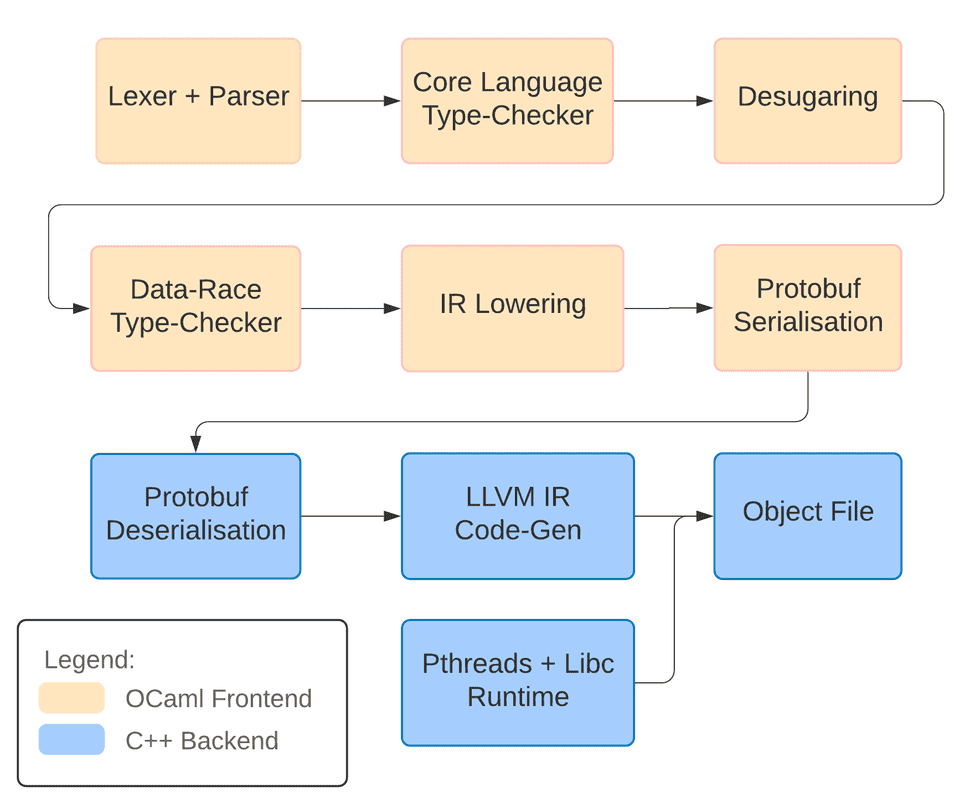
\includegraphics[width=\linewidth]{How I wrote my own proper programming language_files/compiler-pipeline.png}

%
%
%\begin{itemize}
%\item
%  \textbf{Part 1: How I wrote my own "proper" programming language}
%\item
%  { Part 2:
%  }\href{https://mukulrathi.com/create-your-own-programming-language/compiler-engineering-structure/}{So
%  how do you structure a compiler project?}
%\item
%  { Part 3:
%  }\href{https://mukulrathi.com/create-your-own-programming-language/parsing-ocamllex-menhir/}{Writing
%  a Lexer and Parser using OCamllex and Menhir}
%\item
%  { Part 4:
%  }\href{https://mukulrathi.com/create-your-own-programming-language/intro-to-type-checking/}{An
%  accessible introduction to type theory and implementing a
%  type-checker}
%\item
%  { Part 5:
%  }\href{https://mukulrathi.com/create-your-own-programming-language/data-race-dataflow-analysis/}{A
%  tutorial on liveness and alias dataflow analysis}
%\item
%  { Part 6:
%  }\href{https://mukulrathi.com/create-your-own-programming-language/lower-language-constructs-to-llvm/}{Desugaring
%  - taking our high-level language and simplifying it!}
%\item
%  { Part 7:
%  }\href{https://mukulrathi.com/create-your-own-programming-language/protobuf-ocaml-cpp-tutorial/}{A
%  Protobuf tutorial for OCaml and C++}
%\item
%  { Part 8:
%  }\href{https://mukulrathi.com/create-your-own-programming-language/llvm-ir-cpp-api-tutorial/}{A
%  Complete Guide to LLVM for Programming Language Creators}
%\item
%  { Part 9:
%  }\href{https://mukulrathi.com/create-your-own-programming-language/concurrency-runtime-language-tutorial/}{Implementing
%  Concurrency and our Runtime Library}
%\item
%  { Part 10:
%  }\href{https://mukulrathi.com/create-your-own-programming-language/generics-parametric-polymorphism/}{Generics
%  - adding polymorphism to Bolt}
%\item
%  { Part 11:
%  }\href{https://mukulrathi.com/create-your-own-programming-language/inheritance-method-overriding-vtable/}{Adding
%  Inheritance and Method Overriding to Our Language}
%\end{itemize}
%
%\begin{center}\rule{0.5\linewidth}{0.5pt}\end{center}

The diagram above is the compiler for the language Bolt we'll be
building. What do all the stages mean? I have to learn OCaml and C++?
Wait I haven't even heard of OCaml\ldots{}

\textbf{Don't worry.} When I started this project 6 months ago, I had
never built a compiler, nor had I used OCaml or C++ in any serious
project. I'll explain everything in due course.

In this series of posts we'll be building a \emph{proper} programming
language. One of the gripes I had when seeing programming language
tutorials that created a toy language with only operations like addition
and multiplication, was: okay, \emph{but what about a real language like
Java}?

So that's what this series aims to fix. The language Bolt I wrote as
part of my third year disseration is a Java-style concurrent
object-oriented language. Some of the highlights of this series:

\begin{itemize}
\tightlist
\item
  We implement \textbf{objects} and classes, with inheritance and method
  overriding
\item
  \textbf{Concurrency} (as far as I could tell when writing this, no
  other programming language tutorial covered this)
\item
  \textbf{Generics}: being able to write a class of type
  \texttt{LinkedList\textless{}T\textgreater{}} and then instantiating
  it with \texttt{LinkedList\textless{}int\textgreater{}},
  \texttt{LinkedList\textless{}Person\textgreater{}} and so on.
\item
  An introduction to how types are checked in a compiler
\item
  Compiling to LLVM (this post was \#2 on Hacker News!) - LLVM is used
  by C, C++, Swift, Rust amongst many other languages.
\end{itemize}

So I'd encourage you to follow the links in the ``Series'' overview to
learn about these specific features. The remainder of this post will be
to convince you why writing your own programming language is worthwhile,
and the next post will outline the structure of a compiler.

\hypertarget{why-should-you-write-your-own-programming-language}{%
\section{\texorpdfstring{\protect\hyperlink{why-should-you-write-your-own-programming-language}{}Why
should you write your own programming
language?}{Why should you write your own programming language?}}\label{why-should-you-write-your-own-programming-language}}

The question we should really be asking is \emph{why design your own
language}? Possible answers:

\begin{enumerate}
\tightlist
\item
  It's fun
\item
  It's cool to have your own programming language
\item
  It's a good side-project
\end{enumerate}

\hypertarget{mental-models}{%
\section{\texorpdfstring{\protect\hyperlink{mental-models}{}Mental
Models}{Mental Models}}\label{mental-models}}

Whilst all three of these (or none!) might be true, there's a bigger
motivation: having the right \textbf{mental models}. See, when you learn
your first programming language, you view programming through the lens
of that language. Fast forward to your second language, and it seems
hard, you have to relearn syntax and this new language does things
differently. Using more programming languages, you realise that the
languages share common themes. Java and Python have objects, Python and
JavaScript don't require you to write types, the list goes on. Diving
further into programming language theory, you read about the language
constructs present - Java and Python are \emph{object-oriented}
programming languages and Python and JavaScript are
\emph{dynamically-typed}.

The programming languages you've been using actually build upon the
ideas present in older languages that you may not have have heard of.
Simula and Smalltalk introduced the concept of object-oriented
programming languages. Lisp introduced the concept of dynamic typing.
And there are newer research languages coming all the time that
introduce new concepts. A more mainstream example: Rust builds
\textbf{memory-safety} into a low-level systems programming language.

Building your own language (especially if you're adding new ideas) helps
you think more \textbf{critically} about language design, so when you go
learn a new language it's much easier. For example, I had never
programmed in Hack before my internship at Facebook last summer, but
knowing these programming language concepts made it much easier to pick
up.

\hypertarget{what-are-compilers}{%
\section{\texorpdfstring{\protect\hyperlink{what-are-compilers}{}What
are compilers?}{What are compilers?}}\label{what-are-compilers}}

So you've designed your fancy new language and it is going to
revolutionise the world, but there's one problem. \textbf{How do you run
it?} That's the role of a compiler. To explain how compilers work, let's
first flash our minds back to the 19th Century, in the age of the
telegraph. Here we have this fancy new telegraph but how do we send
messages? \textbf{Same problem, different domain.} The telegraph
operator needs to take in speech and convert it to Morse code, and tap
out the code. The first thing the operator does is make sense of the
speech - they split it into words (\textbf{lexing}) , and then
understand how those words are used in a sentence (\textbf{parsing}) -
are they part of a noun phrase, a subordinate clause etc. They check if
it makes sense by classifying words into categories or \textbf{types}
(adjective, noun, verb) and check the sentence makes grammatical sense
(we can't use ``runs'' to describe a noun as it is a verb not a noun).
Finally, they translate (\textbf{compile}) each word into dots and dashs
(Morse code), which is then transmitted along the wire.

This seems like it labours the point, because so much of this is
\emph{automatic} for humans. Compilers work the same way, except we have
to explicitly program computers to do this. The example above describes
a simple compiler consisting of 4 stages: lex, parse, type-check and
then translate into machine instructions. The operator also needs some
additional tools to actually tap out the Morse code; for programming
languages, this is the \textbf{runtime environment}.

In practice, the operator likely constructs some shorthand notation that
they know how to translate to Morse code. Now rather than converting
speech into Morse code directly, they convert the speech into their
shorthand, and then convert the shorthand into Morse code. In many
practical languages, you can't just go directly from the source code to
the machine code, you have \emph{desugaring} or \emph{lowering} stages,
where you remove language constructs stage-by-stage (e.g. unrolling for
loops) until we're left with a small set of instructions that can be
executed. Desugaring makes later stages much easier, as they operate on
a simpler representation. The compiler stages are grouped into frontend,
middle-end and backend, where frontend does much of the
parsing/type-checking, and middle-end and backend simplify and optimise
the code.

\hypertarget{compiler-design-choices}{%
\subsection{\texorpdfstring{\protect\hyperlink{compiler-design-choices}{}Compiler
Design
Choices}{Compiler Design Choices}}\label{compiler-design-choices}}

We can actually frame a lot of language and compiler design in terms of
the analogy above:

Does the operator translate words on-the-fly into Morse code as they
transmit them, or do they convert the words into Morse code beforehand,
and then transmit the Morse code? \textbf{Interpreted} languages like
Python do the former, whilst ahead-of-time \textbf{compiled} languages
like C (and Bolt) do the latter. Java actually lies somewhere in between
- it uses a \textbf{just-in-time} compiler which does most of the work
beforehand, translating programs to bytecode and then at runtime
compiles bytecode to machine code.

Now consider a scenario where a new Lorse code came out that was an
alternative to Morse code. If the operators are taught how to convert
the shorthand to Lorse code, the person speaking doesn't need to know
how that's done, they get it for free. Likewise, a person speaking a
different language just needs to tell the operator how to translate it
to the shorthand, and then they get translations into Lorse \emph{and}
Morse code! This is how \textbf{LLVM} works. \textbf{LLVM IR}
(intermediate representation) acts as the stepping stone that lies
between the program and the machine code. C, C++, Rust and a whole host
of other languages (including Bolt) target LLVM IR, which then compiles
code to a variety of machine architectures.

{
\href{https://mukulrathi.com/static/cf22553f4c173ee4b0dec6bd67e38110/c658e/llvm.png}{{}
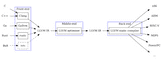
\includegraphics[width=\linewidth]{How I wrote my own proper programming language_files/llvm.png}}
}

Static vs dynamic typing? In the first case, the operator either checks
that the words make grammatical sense before they start tapping. Or,
they don't and then midway through they're like ``huh, this doesn't make
sense'' and stop. Dynamic typing can be seen as quicker to experiment in
(like Python, JS) but when you send that message you don't know if the
operator will stop midway through (crash).

I've explained it in terms of an imaginary telegraph operator, but any
analogy works. Building up this intuition goes a long way in
understanding which language features are right for your language: if
you're going to be experimenting, then maybe dynamic typing is better as
you can move faster. If you're using a larger codebase, it's harder to
proof-read it all and you're more likely to make errors so you probably
should shift towards static typing to avoid breaking things.

\hypertarget{types}{%
\subsection{\texorpdfstring{\protect\hyperlink{types}{}Types}{Types}}\label{types}}

The most interesting part of the compiler (in my opinion) is the
type-checker. In our analogy, the operator classified words as
parts-of-speech (adjectives, nouns, verbs) then checked if they were
used correctly. Types work the same way, we classify program values
based on the behaviour we'd like them to have. E.g. \texttt{int} for
numbers that can be multiplied together, \texttt{String} for streams of
characters that can be concatenated together. The role of the
type-checker is to prevent undesirable behaviour from happening - like
concatenating \texttt{int}s or multiplying \texttt{String}s together -
these operations make no sense so shouldn't be allowed. With type
\emph{checking}, the programmer annotates values with types, and the
compiler checks if they're correct. With type \emph{inference}, the
compiler both infers and checks the types. We call the rules that check
the types \emph{typing judgements}, and a collection of these (along
with the types themselves) forms a type system.

It turns out actually that there's a lot more you can do: type systems
don't just check if \texttt{int}s or \texttt{String}s are used
correctly. Richer type systems can prove stronger invariants about
programs: that they will terminate, access memory safely, or that they
do not contain data races. Rust's type system for example guarantees
memory safety and data-race freedom, as well as checking traditional
types \texttt{int}s and \texttt{String}s.

%\hypertarget{i-make-content-about-my-software-engineering-journey-curated-in-my-newsletter}{%
%\subsection{I make content about my software engineering journey,
%curated in my
%newsletter!}\label{i-make-content-about-my-software-engineering-journey-curated-in-my-newsletter}}
%
%Tips from my time at Cambridge and Facebook, and early access to
%technical tutorials on machine learning, compilers and beyond.
%
%\href{https://newsletter.mukulrathi.com/}{Check out previous issues!}
%
%Email Address
%
%By subscribing, you agree with Revue's
%\href{https://www.getrevue.co/terms}{Terms of Service} and
%\href{https://www.getrevue.co/privacy}{Privacy Policy}.

\hypertarget{where-does-bolt-fit-in}{%
\section{\texorpdfstring{\protect\hyperlink{where-does-bolt-fit-in}{}Where
does Bolt fit
in?}{Where does Bolt fit in?}}\label{where-does-bolt-fit-in}}

Programming languages still haven't cracked the problem of writing safe
concurrent code. Bolt, like Rust, prevents data races
(\href{https://doc.rust-lang.org/nightly/nomicon/races.html}{explained
in this Rust doc}), but takes a more fine-grained approach to
concurrency. Before keyboard warriors come at me on Twitter, I think
Rust has done a brilliant job in getting the conversation about this
going - whilst Bolt will likely never go mainstream, it's demonstrating
another approach.

If we look back at the pipeline now, you can see that Bolt contains the
lexing, parsing, and desugaring/lowering phases. It also contains a
couple of Protobuf serialisation and deserialisation phases: these are
purely to convert between OCaml and C++. It targets LLVM IR, and then we
link in a couple of runtime libraries (pthreads and libc) and finally we
output our \emph{object file}, a binary containing the machine code.

{
\href{https://mukulrathi.com/static/67552b3afe850eb6515a639276f98f47/7792f/compiler-pipeline.png}{{}
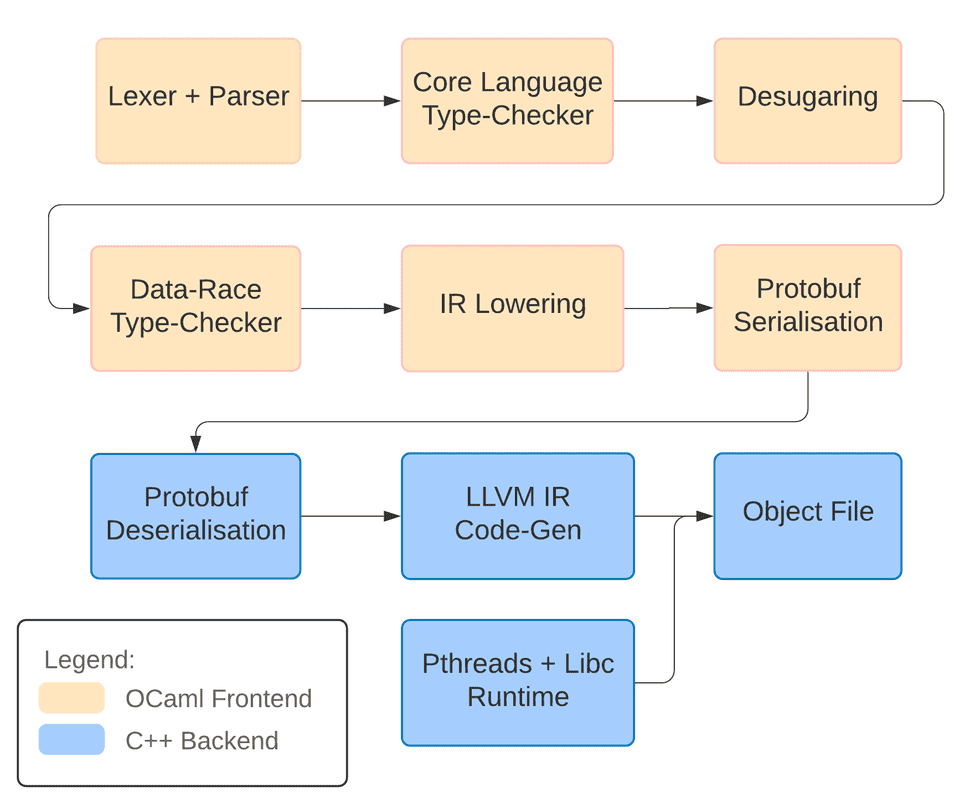
\includegraphics[width=\linewidth]{How I wrote my own proper programming language_files/compiler-pipeline.png}}
}

Unlike most compilers though, Bolt has not one but \textbf{two}
type-checking phases! Bolt has both traditional types and
\textbf{capabilities}, which are, informally, another set of types to
type-check data races. I've
\href{https://github.com/mukul-rathi/bolt-dissertation}{written up a
dissertation} that explores this more formally, if you are interested in
the theory, if not you can skip the data-race checking posts in this
series. We type-check the traditional types first, simplify the language
a bit in the desugaring stage, then do the data-race type-checking.

\hypertarget{and-what-about-this-series}{%
\section{\texorpdfstring{\protect\hyperlink{and-what-about-this-series}{}And
what about this
series?}{And what about this series?}}\label{and-what-about-this-series}}

This series can be thought of from two perspectives: firstly, we will be
discussing language design and comparing Bolt with Java, C++ and other
languages along the way. Secondly, it is a practical step-by-step
tutorial on building your own compiler. Unlike many
build-your-own-compiler tutorials that tell you how to build a
\emph{toy} language, some of the topics this tutorial looks at form the
basis of concurrent object-oriented languages like Java: how classes are
implemented, how inheritance works, generic classes, and even how
concurrency is implemented under the hood.

Bolt also doesn't output toy instructions but instead targets
\textbf{LLVM IR}. Practically speaking, this means Bolt hooks into the
amazing optimisations present in C/C++ compilers. The LLVM API is
powerful, but it's also very hard to navigate the documentation. I spent
many long nights reverse-engineering C++ programs - hopefully this
series prevents at least one person from going through that pain!

In the next part, we'll look at the practical aspects of setting up a
compiler project - I'll walk through the
\href{https://github.com/mukul-rathi/bolt}{Bolt repository} and explain
\emph{why} we're using OCaml of all languages for the frontend.

%\hypertarget{share-this-on-twitter}{%
%\subsection{Share This On Twitter}\label{share-this-on-twitter}}
%
%If you liked this post, please consider sharing it with your network. If
%you have any questions, tweet away and I'll answer :) I also tweet when
%new posts drop!
%
%\textbf{PS:} I also share helpful tips and links as I'm learning - so
%you get them \textbf{well before} they make their way into a post!
%
%\includegraphics[width=1.04167in,height=1.11458in]{How I wrote my own proper programming language_files/profile-pic.png}
%
%\hypertarget{series-creating-the-bolt-compiler-1}{%
%\section{Series: Creating the Bolt
%Compiler}\label{series-creating-the-bolt-compiler-1}}
%
%\begin{itemize}
%\item
%  \textbf{Part 1: How I wrote my own "proper" programming language}
%\item
%  { Part 2:
%  }\href{https://mukulrathi.com/create-your-own-programming-language/compiler-engineering-structure/}{So
%  how do you structure a compiler project?}
%\item
%  { Part 3:
%  }\href{https://mukulrathi.com/create-your-own-programming-language/parsing-ocamllex-menhir/}{Writing
%  a Lexer and Parser using OCamllex and Menhir}
%\item
%  { Part 4:
%  }\href{https://mukulrathi.com/create-your-own-programming-language/intro-to-type-checking/}{An
%  accessible introduction to type theory and implementing a
%  type-checker}
%\item
%  { Part 5:
%  }\href{https://mukulrathi.com/create-your-own-programming-language/data-race-dataflow-analysis/}{A
%  tutorial on liveness and alias dataflow analysis}
%\item
%  { Part 6:
%  }\href{https://mukulrathi.com/create-your-own-programming-language/lower-language-constructs-to-llvm/}{Desugaring
%  - taking our high-level language and simplifying it!}
%\item
%  { Part 7:
%  }\href{https://mukulrathi.com/create-your-own-programming-language/protobuf-ocaml-cpp-tutorial/}{A
%  Protobuf tutorial for OCaml and C++}
%\item
%  { Part 8:
%  }\href{https://mukulrathi.com/create-your-own-programming-language/llvm-ir-cpp-api-tutorial/}{A
%  Complete Guide to LLVM for Programming Language Creators}
%\item
%  { Part 9:
%  }\href{https://mukulrathi.com/create-your-own-programming-language/concurrency-runtime-language-tutorial/}{Implementing
%  Concurrency and our Runtime Library}
%\item
%  { Part 10:
%  }\href{https://mukulrathi.com/create-your-own-programming-language/generics-parametric-polymorphism/}{Generics
%  - adding polymorphism to Bolt}
%\item
%  { Part 11:
%  }\href{https://mukulrathi.com/create-your-own-programming-language/inheritance-method-overriding-vtable/}{Adding
%  Inheritance and Method Overriding to Our Language}
%\end{itemize}
%
%\begin{itemize}
%\item ~
%  \hypertarget{a-step-by-step-guide-to-integrating-reasonml-into-your-gatsby-site}{%
%  \subsection{\texorpdfstring{\href{https://mukulrathi.com/gatsby-reasonml-tutorial/}{←
%  A step-by-step guide to integrating ReasonML into your Gatsby
%  site}}{← A step-by-step guide to integrating ReasonML into your Gatsby site}}\label{a-step-by-step-guide-to-integrating-reasonml-into-your-gatsby-site}}
%\item ~
%  \hypertarget{so-how-do-you-structure-a-compiler-project}{%
%  \subsection{\texorpdfstring{\href{https://mukulrathi.com/create-your-own-programming-language/compiler-engineering-structure/}{So
%  how do you structure a compiler project?
%  →}}{So how do you structure a compiler project? →}}\label{so-how-do-you-structure-a-compiler-project}}
%\end{itemize}
%
%\hypertarget{table-of-contents}{%
%\section{Table of Contents}\label{table-of-contents}}
%
%\href{https://mukulrathi.com/create-your-own-programming-language/intro-to-compiler/\#top-of-page}{}
%
%\hypertarget{how-i-wrote-my-own-proper-programming-language}{%
%\subsection{How I wrote my own "proper" programming
%language}\label{how-i-wrote-my-own-proper-programming-language}}
%
%\begin{itemize}
%\item
%  \href{https://mukulrathi.com/create-your-own-programming-language/intro-to-compiler/\#why-should-you-write-your-own-programming-language}{}
%
%  \hypertarget{why-should-you-write-your-own-programming-language-1}{%
%  \subsection{Why should you write your own programming
%  language?}\label{why-should-you-write-your-own-programming-language-1}}
%\item
%  \href{https://mukulrathi.com/create-your-own-programming-language/intro-to-compiler/\#mental-models}{}
%
%  \hypertarget{mental-models-1}{%
%  \subsection{Mental Models}\label{mental-models-1}}
%\item
%  \href{https://mukulrathi.com/create-your-own-programming-language/intro-to-compiler/\#what-are-compilers}{}
%
%  \hypertarget{what-are-compilers-1}{%
%  \subsection{What are compilers?}\label{what-are-compilers-1}}
%
%  \begin{itemize}
%  \item
%    \href{https://mukulrathi.com/create-your-own-programming-language/intro-to-compiler/\#compiler-design-choices}{}
%
%    \hypertarget{compiler-design-choices-1}{%
%    \subsection{Compiler Design
%    Choices}\label{compiler-design-choices-1}}
%  \item
%    \href{https://mukulrathi.com/create-your-own-programming-language/intro-to-compiler/\#types}{}
%
%    \hypertarget{types-1}{%
%    \subsection{Types}\label{types-1}}
%  \end{itemize}
%\item
%  \href{https://mukulrathi.com/create-your-own-programming-language/intro-to-compiler/\#where-does-bolt-fit-in}{}
%
%  \hypertarget{where-does-bolt-fit-in-1}{%
%  \subsection{Where does Bolt fit
%  in?}\label{where-does-bolt-fit-in-1}}
%\item
%  \href{https://mukulrathi.com/create-your-own-programming-language/intro-to-compiler/\#and-what-about-this-series}{}
%
%  \hypertarget{and-what-about-this-series-1}{%
%  \subsection{And what about this
%  series?}\label{and-what-about-this-series-1}}
%\end{itemize}
%
%© 
%
%\hypertarget{gatsby-announcer}{}
%Navigated to How I wrote my own "proper" programming language
